\subsection{Диффеоморфизм}

\deff{def:} $f: O_1 \subset R^m \rightarrow O_2 \subset \R^m$, $O_1,O_2$ - открытое. $f$ - \deff{диффеоморфизм} между $O_1,O_2$, если
\begin{enumerate}
    \item $f$ - биекция
    \item $f$ - дифф.
    \item $f^{-1}$ - дифф.
\end{enumerate}

\deff{def:} \deff{Область} = открытое связное множество (лин. связное)

Естественно требовать, чтобы $O_1, O_2$ были областями. 




\thmm{Лемма (о бесконечно малых в определении дифф-ти)} или по-другому

\thmm{Лемма (о приближенных значениях дифференцируемого отображения)}

$F: O \subset \R^m \rightarrow \R^m$ ($O$ - открыто - ?)
\begin{enumerate}
    \item $F$ - дифф. в $x_0$, $\det F'(x_0) \neq 0$ (т.е $F'(x_0)$ - обратимый). Тогда: $$\exists c>0,\delta > 0: \forall h: |h|<\delta : |F(x_0+ h)-F(x_0)| > c|h|$$
    \item $F \in C^1(O, \R^m)$. Тогда:
    $$|F(x_0+h)-F(x_0)-F'(x_0)h|\leq M \cdot |h|$$
    где $M = \sup\limits_{x \in [x_0,x_0+h]} ||F'(x) - F'(x_0)||$
\end{enumerate}

\textbf{Доказательство:}
\begin{enumerate}
    \item Пусть $F$ - линейное отображение (линейный оператор). 
    У него производный оператор это матрица $F$. Воспользуемся этим и получим:
    $$\forall h : h = F^{-1}Fh : |h| \leq ||F^{-1}|||Fh| = ||F^{-1}|||F(x+h)-F(x)|$$
    То есть $|F(x+h)-F(x)| \geq |h| \cdot \cfrac{1}{||F^{-1}||} = |h| \cdot c$

    Теперь общий случай: 
    $$|F(x_0 + h)-F(x_0)| = |F'(x_0)h + \alpha(h) |h|| \geq c\cdot |h| - |\alpha(h)| \cdot |h|$$
    Откуда $\exists \delta : \forall h: |h|<\delta : (\alpha(h))<\cfrac{c}{2}$ и $c\cdot |h| - |\alpha(h)| \cdot |h| \geq \cfrac{c}{2}|h|$

\item 

$T(x) = F(x) -F'(x_0) x$, $T'(x) = F'(x) - F'(x_0)$
$$|F(x_0+ h)-F(x_0) - F'(x_0) h| =| T(x_0+h)-T(x_0)| \leq \sup\limits_{x \in [x_0,x_0+h]}||F'(x)-F'(x_0)|| \cdot | h|$$
В конце мы воспользовались теоремой Лагранжа:
$$|F(x_0+h) - F(x_0)|\leq \sup\limits_{x\in[x_0,x_0 + h]} ||F'(x) || \cdot |h|$$

\end{enumerate}

\hfill Q.E.D.

\thmm{Теорема (о сохранении области)}

$F: O\subset \R^m \rightarrow \R^m$, дифф, $\forall x : \det F'(x) \neq 0$, $O$  - открыто. Тогда $F(O)$ - открыто.

\textbf{Доказательство:}

$x_0 \in O, y_0 = F(x_0) \in F(O)$, мы хотим проверить, что $y_0$ - внутренняя точка.

По Лемме выше п.1 $\exists c,\delta >0: \forall h \in \overline{B}(o,\delta): |F(x_0+h) -F(x_0)| \geq C|h| $. Возьмем шар замкнутый (мы можем так сделать, просто описав этот шар, открытым размера чуть больше)

В частности: при $h:|h| \leq \delta :  F(x_0 + h)\neq F(x_0)$.

Введу $r: = \frac{1}{2}dist (y_0, F(S(x_0,\delta))$, где $S(x_0,\delta)$ - сфера: $\{x_0 + h, |h| = \delta\}$.

Так теперь давайте немного остановимся и разъясним че происходит:

$dist := \inf (\rho(y_0, z), z \in (F(S)))$. При этом у нас непрерывная  функция на компакте, следовательно переводит компакт в компакт, а по теореме Вейерштрасса минимум на компакте будет достигаться, то есть $\inf$ можно заменить на $\min$. Может возникнуть 2 случая: $y_0$ лежит внутри или снаружи $F(S)$ и в обоих случае на рисунке показано это расстояние:
\begin{center}
   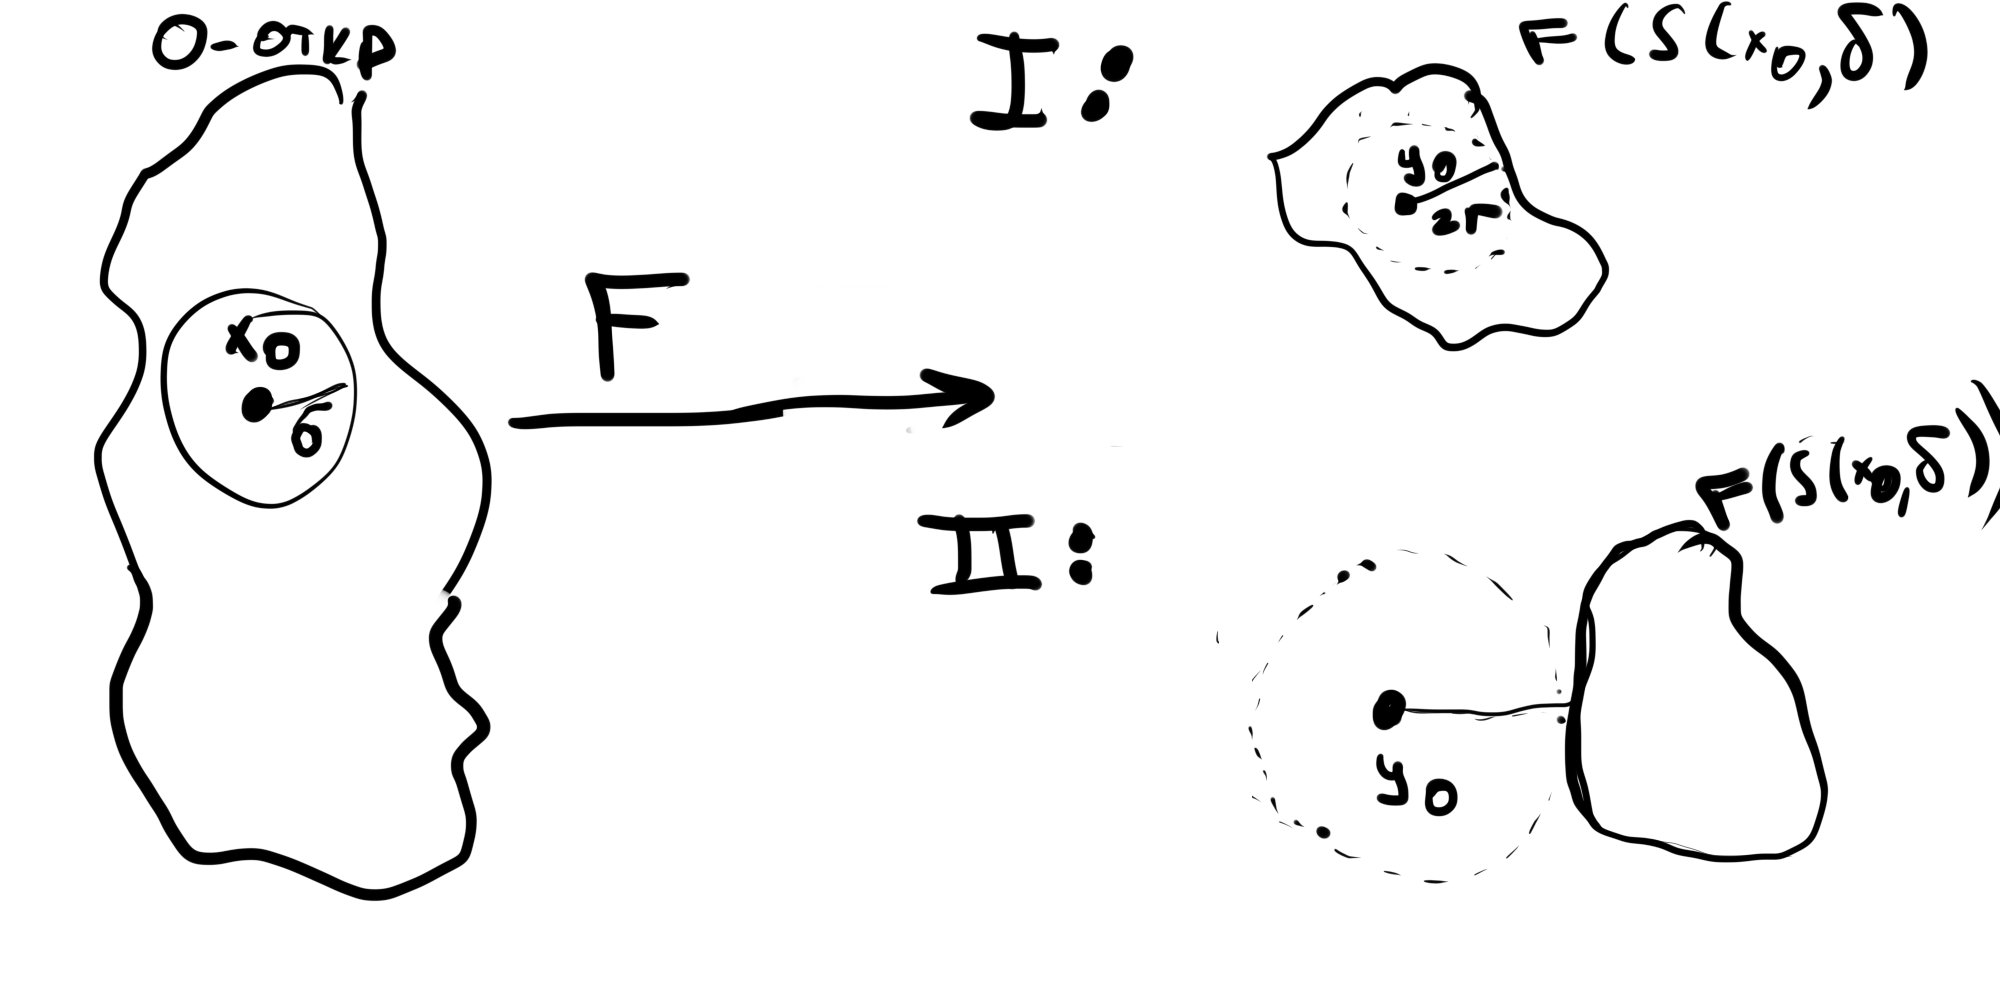
\includegraphics[width=14cm]{assets/block_hard_1.png}
\end{center}
При этом $r > 0$, так как $F(x_0+h) \neq F(x_0)$. Теперь покажем, что $B(y_0,r) \subset  F(O)$.

Докажем: $\forall y: |y-y_0|<r: \exists x\in B(x_0,\delta): F(x) = y$. 

Как только я это проверю, мы сразу получим, что $B(y_0,r) \subset  F(O)$.

Рассмотрим $g(x) = |F(x)-y|^2$ - функция на шаре $\overline{B(x_0,\delta)}$

Этот шар --- компакт и достигает своего минимума внутри шара: при $x \in S(x_0,\delta):g(x) >r^2$, при $x = x_0: g(x)<r^2$.

Тогда точка $\min$ удовлетворяет теореме Ферма:
$$g(x) = \sum\limits_{i=1}^m (F_i(x)-y_i)^2$$. 
Тогда напишем необходимое условие экстремума:
$$\begin{cases}
    \cfrac{\delta g}{\delta x_1}=0: \sum\limits_{i=1}^m 2 (F_i(x)-y_i)\cfrac{\delta F_i(x)}{\delta x_1}=0\\
    \vdots \\
    \cfrac{\delta g}{\delta x_m}=0: \sum\limits_{i=1}^m 2 (F_i(x)-y_i)\cfrac{\delta F_i(x)}{\delta x_m}=0
\end{cases}$$
$$F'(x) \cdot 2(F(x)-y) = 0$$
А значит, так как $\det F'\neq 0$, то $F(x) = y$ и мы нашли такой $x$.

\hfill Q.E.D.

\textbf{Замечание 1:} $F$ - непр, $O$ - связно, $F(O)$ - связно.

\textbf{Замечание 2:} Непрерывность: $\forall$ откр. $O'$ $F^{-1}(O)$ - откр.

\textbf{Следствие о сохранении области для отображений в пространство меньшей размерности:} 

$F: O$ - откр. $\subset \R^m \rightarrow \R^l$, $l<m$, $\forall x : \rg F'(x) = l, F \in C^1(O)$. Тогда $F(O)$ - откр.

\textbf{Доказательство:}

Пусть ранг реализуется на столбцах $x_1,\ldots , x_l$. Построим отображение 
$$\overline{F}(x) = \begin{pmatrix}
    F(x_1)\\
    \vdots\\
    F(x_l)\\
    x_{l+1}\\
    \vdots \\
    x_{m}
\end{pmatrix}$$
Возьмем $U(x_0)$, что матрица $\det \overline{F}'(x)$ будет иметь блочно диагональный вид и определитель не ноль, откуда определитель не ноль, можем применить теорему, для нее будет верно сохранение области, получим открытую в $\R^m$ и в первом семестре была теорема, что открытое в $\R^m$ будет открытым в $\R^l$

TODO: причесать русский язык

\hfill Q.E.D


\thmm{Теорема (о гладкости обратного изображения)}

$F: O \subset \R^m \rightarrow \R^m : F \in C^r, \det F'\neq 0$ в $O$, открыто.

Допустим $F$ - обратимо. Тогда $F^{-1}\in C^r$

\textbf{Доказательство:}

На экзамене не просят TODO: 15 лекция 2:33

\hfill Q.E.D.

\thmm{Теорема (о локальной обратимости)}

$F \in O \subset \R^m \rightarrow \R^m, x_0 \in O$, $O$ - открытое. $F \in C^1$

Пусть $\det F'(x_0) \neq 0$. Тогда $\exists U(x_0):F\Big|_{U(0)}$ - диффеоморфизм.

\textbf{Доказательство:}

По лемме о приближенных значениях дифференцируемого отображения, по пункту 1 выбираем  $c$, по пункту 2 выбираем $U(x_0) = B(x_0,r)\subset O$ так, чтобы:
\begin{enumerate}
    \item $\det F'(x) \neq0$, при $x \in U(x_0)$
    \item $||F'(x)-F'(x_0)||< \cfrac{c}{4}$, при $x\in U(x_0)$
\end{enumerate}

\textbf{Замечание от Славы:} Почему такая окрестность существует? По теореме о непрерывно дифференцируемых отображений, наше отображение $F'$ непрерывно. Из-за этого есть окрестность, которая удовлетворяет нашим условиям.


Проверяемость обратимость $F$ на $U(x_0)$: $x,y \in U(x_0), y = x+h: F(y) \neq F(h)$
$$F(y)-F(x)=F(x+h)-F(x) = (F(x+h) - F(x) - F'(x)h) + (F'(x)h - F'(x_0)h) + F'(x_0)h$$
Возьмем норму и воспользуемся:  $|a+ b+ c| = |c|-|b|-|a|$:
$$|F(x+h)-F(x) |=|F'(x_0)h|  -|(F(x+h) - F(x) - F'(x)h)| - |(F'(x)h - F'(x_0)h)| + \geq $$
$$\geq c \cdot |h|  - M \cdot |h| -||F'(x)-F'(x_0)||\cdot|h|\geq c\cdot |h| - M \cdot |h| - \cfrac{c}{4}\cdot h$$
Оценили с помощью леммы и выбора окрестности. Оценим наше $M$ сверху
$$M:=\sup\limits_{z\in [x,x+h]}||F'(z)-F'(x)||\leq\sup\limits_{z\in [x,x+h]}||F'(z)-F'(x_0)|| + \sup\limits_{z\in [x,x+h]}||F'(x_0)-F'(x)|| \leq \cfrac{c}{4}+ \cfrac{c}{4} $$
Откуда $|F(y)-F(x)| = |F(x+h)-F(x)|>0$, откуда $F(x) \neq F(y)$

Откуда $F$ обратимо в данной окрестности. По теореме о гладкости обратного изображения, получаем нужные нам условия для диффеоморфизма. Победили

\hfill Q.E.D.

\thmm{Формулировка теоремы о  локальной обратимости в терминах систем уравнений}

$f_i \in C_1:
\begin{cases}
    f_1(x) = y_1^0\\
    \vdots \\
    f_m(x) = y_n^0
\end{cases}$

Пусть $x_0$ - решение этой системы и оказалось $F'(x_0)\neq 0 $. Тогда $\exists V(y_0): \forall y \in V(y_0): \exists$ $x$ близкий к $x_0$, который является решением вашей системы.

\deff{def:} $F: \R^{m+n}\rightarrow  \R^n, F \longleftrightarrow F(x,y)$, где $x\in \R^m, y\in \R^n$.

\thmm{Теорема (о неявном отображении)}

$F: O \subset \R^{m+n}
\rightarrow  \R^n, F \in C^r, (a,b)\in O, F(a,b) = 0$. Пусть $\det F_y'(a,b) \neq 0$

Тогда:
\begin{enumerate}
    \item $\exists$ откр $P \subset \R^n$, $a\in P$
    \item $\exists$ откр $Q \subset \R^n$, $b \in Q$
    \item $\exists! \varphi: P\rightarrow Q, \varphi \in C^r: \forall x \in P: F(x,\varphi(x)) = 0$
\end{enumerate}

